
%(BEGIN_QUESTION)
% Copyright 2010, Tony R. Kuphaldt, released under the Creative Commons Attribution License (v 1.0)
% This means you may do almost anything with this work of mine, so long as you give me proper credit

Suppose this solenoid-controlled valve remains open all the time no matter which switch is pressed:

$$\includegraphics[width=15.5cm]{i01425x01.eps}$$

You measure 474 volts between terminals {\bf H1} and {\bf H4} on the transformer, and 118 volts between terminals {\bf M} and {\bf D}, with both pushbutton switches unpressed.

Identify the likelihood of each specified fault for this system.  Consider each fault one at a time (i.e. no coincidental faults), determining whether or not each fault could independently account for {\it all} measurements and symptoms in this system.  Also, identify one more possible fault not listed in the table.

% No blank lines allowed between lines of an \halign structure!
% I use comments (%) instead, so that TeX doesn't choke.

$$\vbox{\offinterlineskip
\halign{\strut
\vrule \quad\hfil # \ \hfil & 
\vrule \quad\hfil # \ \hfil & 
\vrule \quad\hfil # \ \hfil \vrule \cr
\noalign{\hrule}
%
% First row
{\bf Fault} & {\bf Possible} & {\bf Impossible} \cr
%
\noalign{\hrule}
%
% Another row
Fuse F3 blown (failed open) &  &  \cr
%
\noalign{\hrule}
%
% Another row
Solenoid coil failed open &  &  \cr
%
\noalign{\hrule}
%
% Another row
``Open'' switch contacts (L to M) failed open &  &  \cr
%
\noalign{\hrule}
%
% Another row
``Close'' switch contacts (J to K) failed shorted &  &  \cr
%
\noalign{\hrule}
%
% Another row
Relay coil failed shorted &  &  \cr
%
\noalign{\hrule}
%
% Another row
Relay contact (G to P) failed shorted &  &  \cr
%
\noalign{\hrule}
%
% Another row
Relay contact (F to N) failed shorted &  &  \cr
%
\noalign{\hrule}
%
% Another row
Wire open between terminals K and D &  &  \cr
%
\noalign{\hrule}
%
% Another row
Valve V1 shut &  &  \cr
%
\noalign{\hrule}
%
% Another row
Valve V2 shut &  &  \cr
%
\noalign{\hrule}
} % End of \halign 
}$$ % End of \vbox

Finally, identify the {\it next} diagnostic test or measurement you would make on this system.  Explain how the result(s) of this next test or measurement help further identify the location and/or nature of the fault.

\underbar{file i01425}
%(END_QUESTION)





%(BEGIN_ANSWER)

% No blank lines allowed between lines of an \halign structure!
% I use comments (%) instead, so that TeX doesn't choke.

$$\vbox{\offinterlineskip
\halign{\strut
\vrule \quad\hfil # \ \hfil & 
\vrule \quad\hfil # \ \hfil & 
\vrule \quad\hfil # \ \hfil \vrule \cr
\noalign{\hrule}
%
% First row
{\bf Fault} & {\bf Possible} & {\bf Impossible} \cr
%
\noalign{\hrule}
%
% Another row
Fuse F3 blown (failed open) &  & $\surd$ \cr
%
\noalign{\hrule}
%
% Another row
Solenoid coil failed open &  & $\surd$ \cr
%
\noalign{\hrule}
%
% Another row
``Open'' switch contacts (L to M) failed open &  & $\surd$ \cr
%
\noalign{\hrule}
%
% Another row
``Close'' switch contacts (J to K) failed shorted & $\surd$ &  \cr
%
\noalign{\hrule}
%
% Another row
Relay coil failed shorted &  & $\surd$ \cr
%
\noalign{\hrule}
%
% Another row
Relay contact (G to P) failed shorted &  & $\surd$ \cr
%
\noalign{\hrule}
%
% Another row
Relay contact (F to N) failed shorted & $\surd$ &  \cr
%
\noalign{\hrule}
%
% Another row
Wire open between terminals K and D &  & $\surd$ \cr
%
\noalign{\hrule}
%
% Another row
Valve V1 shut & ? &  \cr
%
\noalign{\hrule}
%
% Another row
Valve V2 shut &  & $\surd$ \cr
%
\noalign{\hrule}
} % End of \halign 
}$$ % End of \vbox

In order for a ``shut'' V1 to account for the control valve remaining open all the time, that hand valve would have had to be shut while the system was in a very particular condition!  Simply shutting V1 under {\it any} condition(s) would not necessarily produce this effect.

\vskip 10pt

A good ``next test'' would be to measure voltage between terminals Q and R on the solenoid.

%(END_ANSWER)





%(BEGIN_NOTES)

Additional possible faults not listed in the table include:

\begin{itemize}
\item{} Short between terminals A and C 
\item{} Severely plugged silencer
\end{itemize}











\vskip 20pt \vbox{\hrule \hbox{\strut \vrule{} {\bf Virtual Troubleshooting} \vrule} \hrule}

This question is a good candidate for a ``Virtual Troubleshooting'' exercise.  Presenting the diagram to students, you first imagine in your own mind a particular fault in the system.  Then, you present one or more symptoms of that fault (something noticeable by an operator or other user of the system).  Students then propose various diagnostic tests to perform on this system to identify the nature and location of the fault, as though they were technicians trying to troubleshoot the problem.  Your job is to tell them what the result(s) would be for each of the proposed diagnostic tests, documenting those results where all the students can see.

During and after the exercise, it is good to ask students follow-up questions such as:

\begin{itemize}
\item{} What does the result of the last diagnostic test tell you about the fault?
\item{} Suppose the results of the last diagnostic test were different.  What then would that result tell you about the fault?
\item{} Is the last diagnostic test the best one we could do?
\item{} What would be the ideal order of tests, to diagnose the problem in as few steps as possible?
\end{itemize}


%INDEX% Troubleshooting review: electric circuits

%(END_NOTES)


